%LTeX: language=it
\subsection{UC 11 - Eliminare un oggetto} \label{sec:UC3}
    \begin{figure}[h]
        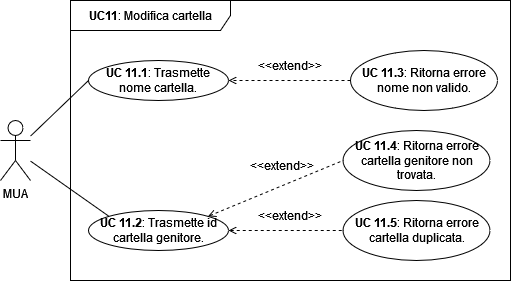
\includegraphics[width=0.85\textwidth]{sections/uc_imgs/UC11.png}
        \centering
        \caption{Diagramma UC11 }
    \end{figure}
    \begin{itemize}
        \item \textbf{Attore principale}: MUA;
        \item \textbf{Descrizione}: il MUA deve poter eliminare un oggetto dal sistema;
        \item \textbf{Precondizioni}: l’account che il MUA gestisce è registrato nel sistema, e ha un connessione aperta con il sistema ed è autenticato;
        \item \textbf{Postcondizioni}: il MUA elimina un oggetto che è stato rimosso dal sistema;
        \item \textbf{Scenario principale}:
            \begin{enumerate}
                \item il MUA invia i dettagli necessari ad indentificare l'oggetto da eliminare al sistema;
                \item il sistema elimina l'oggetto;
            \end{enumerate}
        \item \textbf{Inclusioni}: nessuna;
        \item \textbf{Generalizzazioni}:
            \begin{itemize}
                \item il MUA elimina un contatto (\hyperref[sec:UC12]{UC 12});
                \item il MUA elimina un evento nel calendario (\hyperref[sec:UC13]{UC 13});
                \item il MUA elimina una cartella (\hyperref[sec:UC14]{UC 14});
            \end{itemize}
        \item \textbf{Estensioni}: 
        \begin{itemize}
            \item 
        \end{itemize}
    \end{itemize}

    %     \subsection{UC 3 - Creare un oggetto} \label{sec: UC 3}
%     \begin{itemize}
%         \item Attore: MUA;
%         \item Descrizione: il MUA deve poter creare un oggetto specifico;
%         \item Scenario principale:
%             \begin{enumerate}
%                 \item 
%             \end{enumerate}
%         \item Generalizzazioni:
%             \begin{itemize}
%                 \item il MUA crea una cartella (\hyperref[sec: UC 3.1]{UC 3.1});
%                 \item il MUA crea un contatto (\hyperref[sec: UC 3.2]{UC 3.2});
%                 \item il MUA crea una condivisione (\hyperref[sec: UC 3.3]{UC 3.3});
%                 \item il MUA crea un evento (\hyperref[sec: UC 3.4]{UC 3.4}).
%             \end{itemize}
%         \item Estensioni: errore ;
%         \item Precondizioni: l’account che il MUA gestisce è registrato nel sistema ed è autenticato;
%         \item Postcondizioni: è stato creato l’oggetto desiderato.
%     \end{itemize}